

\spl applies the concept of an AJAX web application, as described in \secref{ajax}.
It consists of several modules which communicate through defined APIs.
\figref{whole_setup} shows an overview of the implemented modules and their communication channels.

\begin{figure}[htbp]
  \centering
    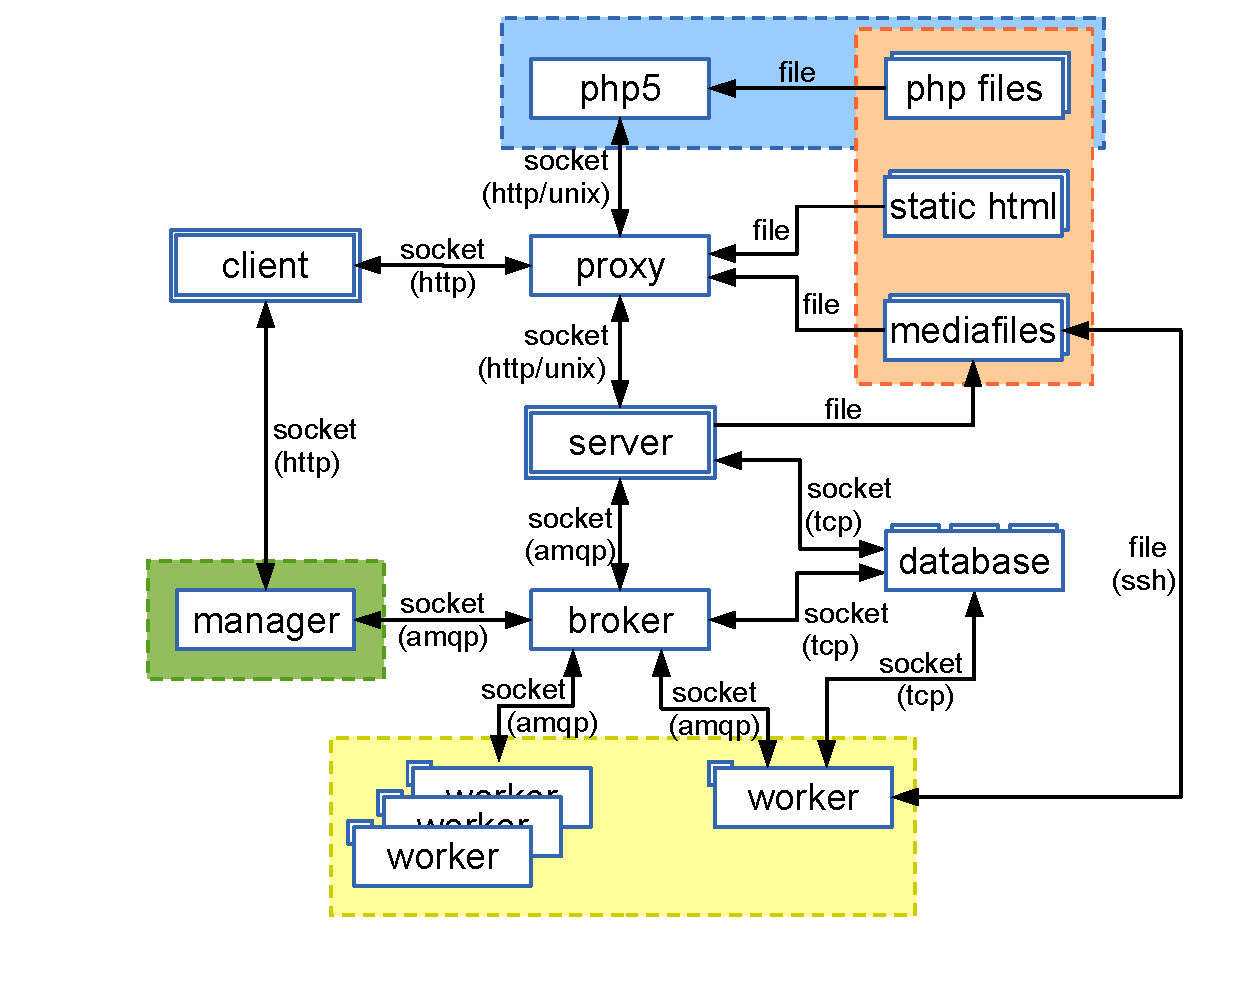
\includegraphics[width=\textwidth]{fig/whole_setup.pdf}
  \caption{Schematics of full \spl setup including communication protocol. Including additional module for hosting additional pages (top blue box) and administrative interface for worker management (left green box). Also showing the file system (top right orange box) and worker nodes running the simulation software (bottom yellow box).}
  \label{fig:whole_setup}
\end{figure}


%This section elaborates the implementation of \spl by explaining design consideration and implementation details for all the modules.
\Figref{whole_setup} shows all modules used in the current setup as an web application at \splurl.
The client, server and worker modules are the core components, needed to run \spl.
Simpler setups are possible. \spl could be run as a native desktop application using only the core modules server and client.

One advantage of this modularized approach is the scalability of the application.
Each module can possibly run on it's own hardware, if the use of the application increases.

The application features a simple flow of data.
After the loading of a Lens into the client application on the browser (client), the user creates a model, which is represented as a JSON string.
This model is sent to the server side application, where the model and all according parameters are saved in a data base.
Additionally, the server creates a configuration file (\T{.cfg} file) which is stored in the file system so that the simulation application (worker) con run on it.
The worker runs the simulation and the resulting set of models is saved to the file system as a State file (\T{.state}).
A second worker step (renderer) then loads this state file and creates the resulting images (mediafiles) and saves them to the file system.
In the current implementation, the simulation and the rendering are done by the same worker.
Future development will feature a separate renderer, in order to allow the creation of arbitrary plots from already simulated data.
In a last step, the client loads the rendered images and gives the user a visual feedback of the model created.

\Figref{dataflow} shows this high level view of data flow.
The sections in this chapter elaborate the interfaces for this data flow, the design of according data structures, as well as the mechanics and implementation of the modules.
\Secref{pd_flow} shows the program and data flows in more detail.

\begin{figure}[htbp]
  \centering
    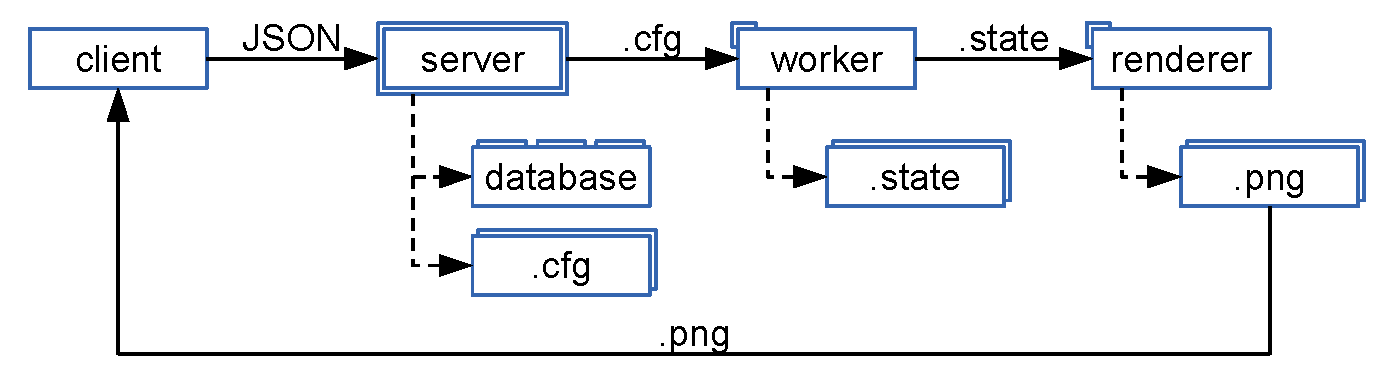
\includegraphics[width=\figwidth]{fig/dataflow.pdf}
  \caption{High level view of flow of data involved in creating a model and data objects saved.}
  \label{fig:dataflow}
\end{figure}



